
\chapter{Tool design}

While the end user executes a single command to apply the \FOLDING tool, this command hides two major components that are executed sequentially and all the outputs are generated into a newly created directory with the name of the input trace-file.
The first component processes a user-given trace-file that contains instrumented and sampled data and generates a textual file that contains sequences of instances and samples.
The second component takes these sequences of instances and samples, then applies the contouring algorithm, any performance model, and the call-stack processing, and, finally, it generates the output results.
Both components are grouped together within the \texttt{folding.sh} appearing to the user that the \FOLDING simply consists of a single tool.
The tool package contains additional components that may be capture the interest of the user.

\section{First component: trace-file processing}

\begin{figure}
  \centering
  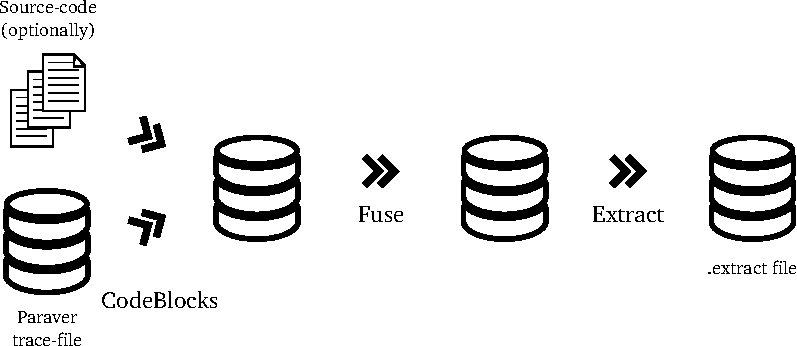
\includegraphics[width=0.5\textwidth]{figures/user-guide/codeblocks-fuse-extract.pdf}
  \caption{Data-flow for the first component of the folding.}
  \label{fig:dataflow_1st_component_folding}
\end{figure}


The first component is divided into three phases that are executed one after another with the user-given trace-file and each of these parse the given trace-file and generates another trace-file that will be used in the subsequent phase as depicted in Figure~\ref{fig:dataflow_1st_component_folding}.
Each of these phases are built in a similar fashion.
They parse the input trace-file and keep in memory information regarding the thread state, and eventually, add information to the output.
The phases are:

\begin{enumerate}

	\item \texttt{codeblocks} (found in \texttt{src/codeblocks})\\
	This phase attributes to each sample information regarding to the loop / code region that it belongs to according to the application source code. 

	\item \texttt{fuse} (found in \texttt{src/fuse})\\
	This phase compacts the trace-file and ensures that the resulting trace-file is well formed.

	\item \texttt{extract} (found in \texttt{src/extract})\\
	This is the final phase and extracts information regarding the instances and samples within the trace-file.

\end{enumerate}

The output of this component is a set of files containing information relative to the application. 
The most notable output is the \texttt{.extract} file, which contains the sequence of instances and their samples.
For instance, Listing~\ref{lst:ExampleGenerationInterpolationOutput} shows the contents of the \texttt{.extract} file generated using the provided example to demonstrate the API facility.
This listing contains information regarding one instance of the \texttt{FunctionA} region.
The instance starts at timestamp 1,000~ns and lasts 4,500~ns, and it executes up to 2,500 instructions (PAPI\_TOT\_INS) and takes 5,000 cycles (PAPI\_TOT\_CYC) to complete.
This instance has two samples associated that ocurred at timestamps 2,000 and 4,000, and each of those provides information regarding the aforementioned performance counters.

\begin{lstlisting}[
 frame=tb,
 basicstyle=\small\ttfamily,
 keywordstyle=\small\bfseries,
 commentstyle=\small\itshape,
 numbers=left,
 firstnumber=1,
 numberstyle=\tiny\color{gray},
 captionpos=t,
 caption={Output example for the extract phase of the \FOLDING mechanism.},
 tabsize=4,
 label=lst:ExampleGenerationInterpolationOutput,
 float=h
]
I 2 2 2 FunctionA 1000 4500 2 PAPI_TOT_CYC 5000 PAPI_TOT_INS 2500
S 2000 1000 2 PAPI_TOT_CYC 2000 PAPI_TOT_INS 1000 0 0
S 4000 3000 2 PAPI_TOT_CYC 4000 PAPI_TOT_INS 2000 2 0 1 2 3 1 3 4 5 0
\end{lstlisting}


\section{Second component: applying the folding}

The main objective of this component relies on processing the instances and samples extracted and generate the output results.
These results include the temporal evolution of the performance counters, any models requested by the user, the source code references and memory references progression, and the results are written in gnuplot and \PARAVER trace files.
This section gives a summarized view of the folding work-flow by depicting the most notable class diagrams found in the application source code.

\begin{figure}
  \centering
  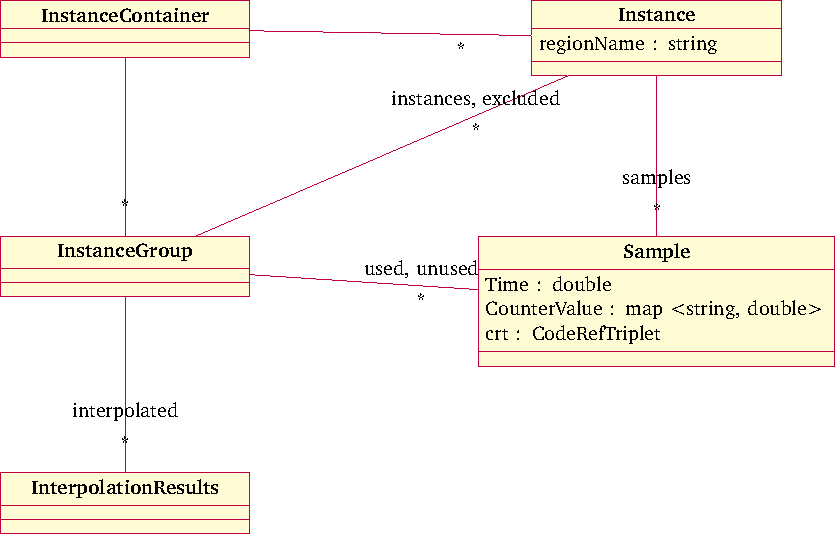
\includegraphics[width=0.80\textwidth]{figures/user-guide/tool-design-interpolate-instances.pdf}
  \caption{Main instances and samples related diagram classes.}
  \label{fig:tool_design_interpolate_instances}
\end{figure}


Figure~\ref{fig:tool_design_interpolate_instances} shows a portion of the classes that are most important within this tool.
The classes \textsl{Instance} and \textsl{Sample} refer to the instances and samples as-is, without any further processing and as generated by the \texttt{extract} tool, in which each \textsl{Instance} contains a set of \textsl{Sample}, and every \textsl{Instance} belongs to an \textsl{InstanceContainer}.

\documentclass{standalone}

\usepackage{tikz}
\usepackage{pgf-umlcd}
\usepackage[bitstream-charter]{mathdesign} % +1! taules mes petites i hi caben
\usepackage[T1]{fontenc}
\usepackage[utf8]{inputenc}

\begin{document}

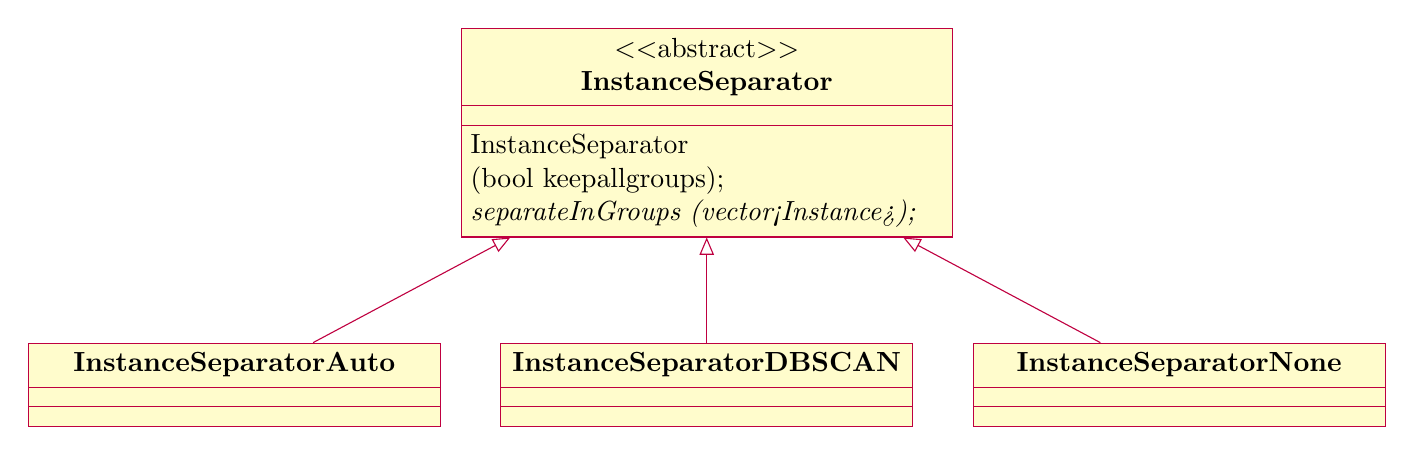
\begin{tikzpicture}

\begin{abstractclass}[text width=6cm]{InstanceSeparator}{0,0}
\operation{InstanceSeparator (bool keepallgroups);}
\operation[0]{separateInGroups (vector<Instance>);}
\end{abstractclass}

\begin{class}[text width=5cm]{InstanceSeparatorAuto}{-6,-4}
\inherit{InstanceSeparator}
\end{class}
\begin{class}[text width=5cm]{InstanceSeparatorDBSCAN}{0,-4}
\inherit{InstanceSeparator}
\end{class}
\begin{class}[text width=5cm]{InstanceSeparatorNone}{6,-4}
\inherit{InstanceSeparator}
\end{class}
\end{tikzpicture}

\end{document}


After reading every \textsl{Instance}, the folding may apply a clustering algorithm (see Figure~\ref{fig:tool_design_interpolate_instance_separator}) according to the duration of each instance in order to reduce the difference between folded \textsl{Instance}.
Currently, there are three alternatives regarding the grouping.

\begin{itemize}

	\item \textsl{InstanceSeparatorNone} groups all instances into a single group.

	\item \textsl{InstanceSeparatorAuto} automatically groups the instances according to their duration. The grouping partitions the time-space interval defined by the shortest and longest instances and looks for group of nearby instances.

	\item \textsl{InstanceSeparatorDBSCAN} groups the instances according to a DBSCAN algorithm applied to the duration of the instances. The DBSCAN algorithm groups together instances that are closely packed together (instances with many nearby neighbors) in terms of time and marks as outliers those instances that lie alone in low-density regions. This grouping uses the ClusteringSuite implementation from the BSC performance tools\footnote{See \url{http://www.bsc.es/computer-sciences/performance-tools/downloads}.}.

\end{itemize}

This grouping begets the \textsl{InstanceGroup} objects which contains references to those \textsl{Instance} that belong to that particular group.
Then, the folding removes the outliers to each \textsl{Instance} within every \textsl{InstanceGroup} and store the outliers and the remaining in the \textit{excluded} and \textit{instances} associations, respectively.

\documentclass{standalone}

\usepackage{tikz}
\usepackage{pgf-umlcd}
\usepackage[bitstream-charter]{mathdesign} % +1! taules mes petites i hi caben
\usepackage[T1]{fontenc}
\usepackage[utf8]{inputenc}

\begin{document}

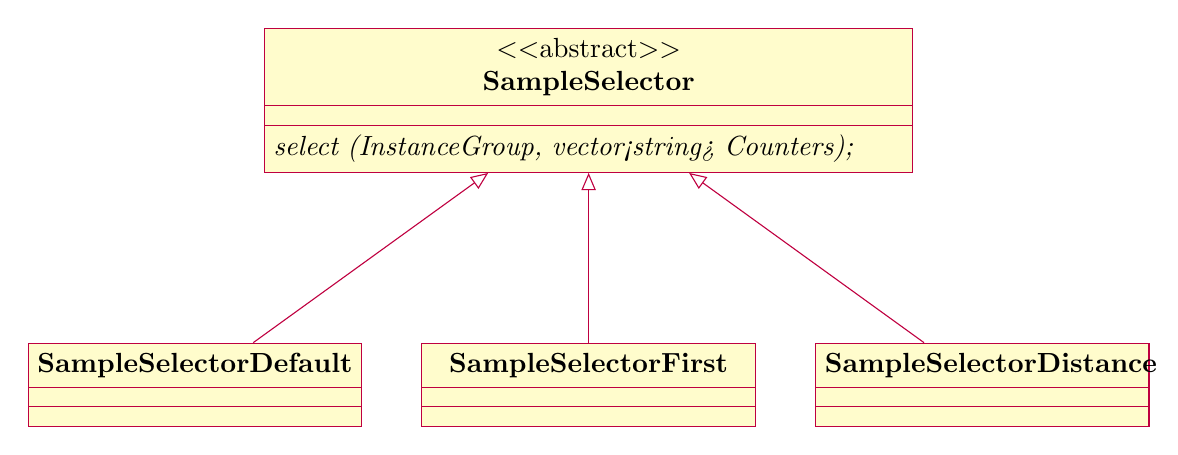
\begin{tikzpicture}

\begin{abstractclass}[text width=8cm]{SampleSelector}{0,0}
\operation[0]{select (InstanceGroup, vector<string> Counters);}
\end{abstractclass}

\begin{class}[text width=4cm]{SampleSelectorDefault}{-5,-4}
\inherit{SampleSelector}
\end{class}
\begin{class}[text width=4cm]{SampleSelectorFirst}{0,-4}
\inherit{SampleSelector}
\end{class}
\begin{class}[text width=4cm]{SampleSelectorDistance}{5,-4}
\inherit{SampleSelector}
\end{class}
\end{tikzpicture}

\end{document}


Since the complexity of the contouring algorithms depends on the number of points to connect, and therefore the number of samples to fold, the \FOLDING tool supports limiting the number of samples given to these algorithms.
Figure~\ref{fig:tool_design_interpolate_sample_selector} depicts the class diagram of the available \textsl{SampleSelector} mechanisms to limit the number of samples.

\begin{itemize}

	\item \textsl{SampleSelectorDefault} the \textit{select} method returns all of the samples within the \textsl{InstanceGroup}. This is useful when the user does not impose any limit to the number of samples to be folded.

	\item \textsl{SampleSelectorFirst} receives a threshold ($N$) in the class constructor. Then, the \textit{select} method tags the first $N$ samples for the processing while the rest are marked as \textit{unused}.

	\item \textsl{SampleSelectorDistance} receives a threshold ($N$) in the class constructor. Then, the \textit{select} method tags $N$ samples that are equidistant within the \textsl{Instance} duration, while the rest are \textit{unused}.

\end{itemize}

\begin{figure}
  \centering
  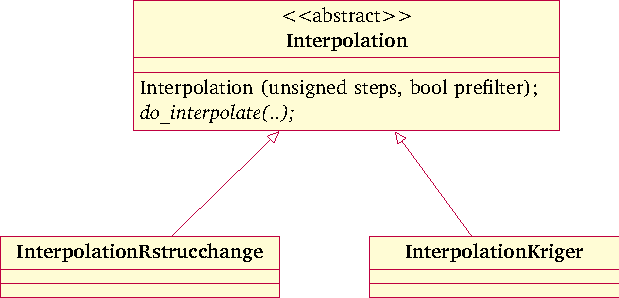
\includegraphics[width=0.50\textwidth]{figures/user-guide/tool-design-interpolate-interpolation.pdf}
  \caption{Performance counter interpolation related diagram classes.}
  \label{fig:tool_design_interpolate_interpolation}
\end{figure}


Then the \FOLDING repeatedly applies the contouring algorithm to the \textit{used} samples among the different \textsl{InstanceGroup} objects.
The contouring algorithm applies to each performance counter individually, and as of writing this document, there are two approaches that honor the \textsl{Interpolation} super-class virtual method (mainly \texttt{do\_interpolate}):

\begin{itemize}

	\item \textsl{InterpolationKriger} uses the self-provided contouring algorithm based on the Kriging mechanism to implement the \texttt{do\_interpolate}.

	\item \textsl{InterpolationRstrucchange} employs the strucchange package\footnote{\url{http://cran.r-project.org/web/packages/strucchange/index.html}} from the R statistical package\footnote{\url{http://www.r-project.org}} to use piece-wise linear regressions to the folded samples. Additionally, this package may benefit from parallel environments if the doParallel package\footnote{\url{http://cran.r-project.org/package=doParallel}} is available on the system.

\end{itemize}

The interpolation results are stored, per performance counter, into \textsl{InterpolationResults} objects that are associated by \textsl{InstanceGroup} by the attribute \textit{interpolated} (as depicted in Figure~\ref{fig:tool_design_interpolate_instances}).
The \textit{interpolated} attribute is implemented as a hash function indexed by the performance counter, so that the interpolation results can be fetched easily.

\documentclass{standalone}

\usepackage{tikz}
\usepackage{pgf-umlcd}
\usepackage[bitstream-charter]{mathdesign} % +1! taules mes petites i hi caben
\usepackage[T1]{fontenc}
\usepackage[utf8]{inputenc}

\begin{document}

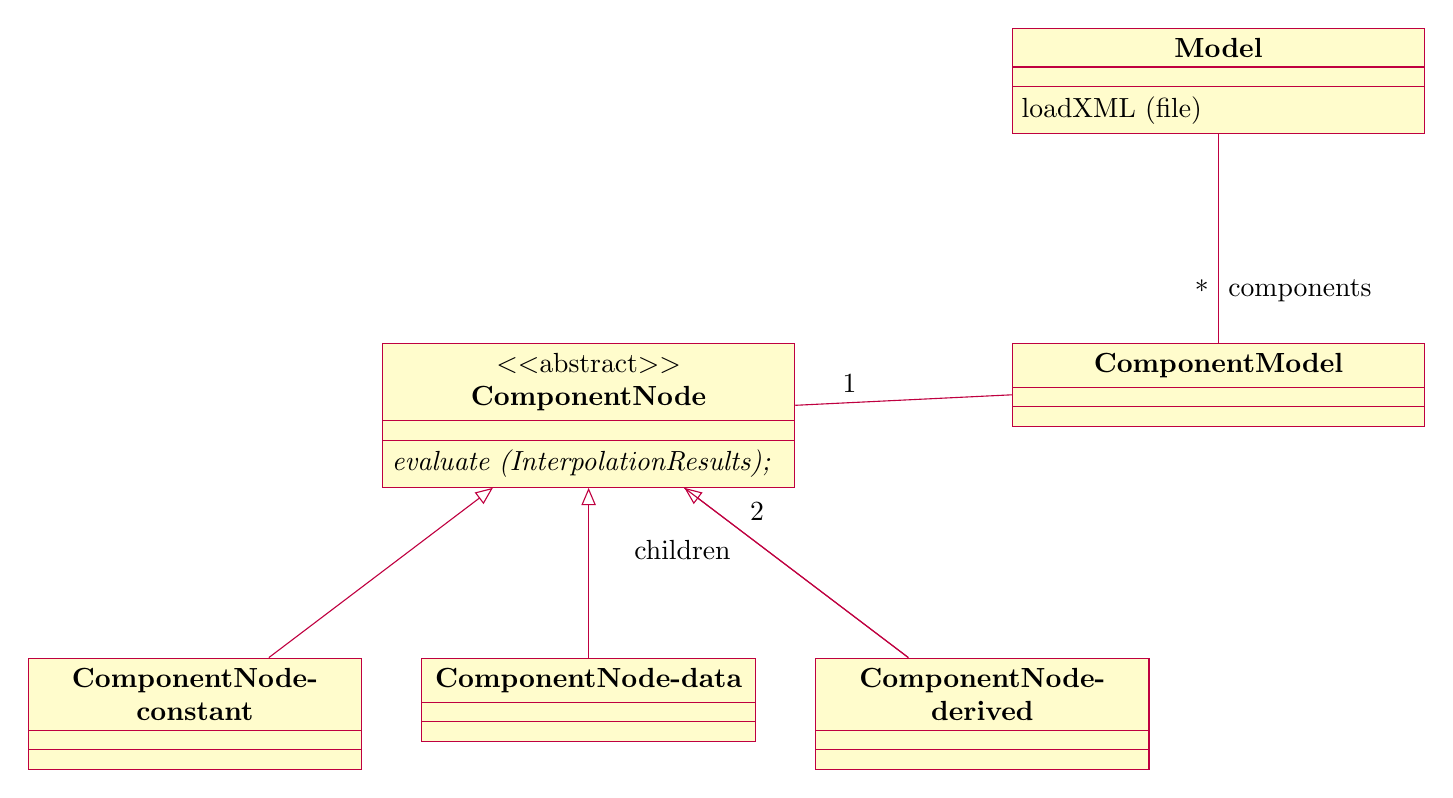
\begin{tikzpicture}

\begin{abstractclass}[text width=5cm]{ComponentNode}{0,0}
\operation[0]{evaluate (InterpolationResults);}
\end{abstractclass}

\begin{class}[text width=4cm]{ComponentNode-constant}{-5,-4}
\inherit{ComponentNode}
\end{class}
\begin{class}[text width=4cm]{ComponentNode-data}{0,-4}
\inherit{ComponentNode}
\end{class}
\begin{class}[text width=4cm]{ComponentNode-derived}{5,-4}
\inherit{ComponentNode}
\end{class}

\association{ComponentNode-derived}{}{}{ComponentNode}{children}{2};

\begin{class}[text width=5cm]{ComponentModel}{8,0}
\end{class}

\association{ComponentModel}{}{}{ComponentNode}{}{1}

\begin{class}[text width=5cm]{Model}{8,4}
\operation{loadXML (file)}
\end{class}

\association{Model}{}{}{ComponentModel}{components}{*}

\end{tikzpicture}

\end{document}


\begin{lstlisting}[
 float=h,
 language=XML,
 frame=tb,
 basicstyle=\small\ttfamily,
 keywordstyle=\small\bfseries,
 commentstyle=\small\itshape,
 numbers=left,
 firstnumber=1,
 numberstyle=\tiny\color{gray},
 captionpos=t,
 caption={Folding example model that generates the L1D and L2D misses per instruction, in addition to the MIPS rate},
 label=lst:Folding_sample_model,
]
<?xml version='1.0'?>

<model name="sample" title-name="Sample model"
       y1="Ratios" y2="MIPS" y1-stacked="no">

    <component name="l1_dcm_ratio" title-name="L1 DCM" where="y1"
               color="red">
        <operation type='/'>
            <value> PAPI_L1_DCM </value>
            <value> PAPI_TOT_INS </value>
        </operation>
    </component>

    <component name="l2_dcm_ratio" title-name="L2 DCM" where="y1"
               color="blue">
        <operation type='/'>
            <value> PAPI_L2_DCM </value>
            <value> PAPI_TOT_INS </value>
        </operation>
    </component>

    <component name="mips" title-name="MIPS" where="y2" color="black">
        <value> PAPI_TOT_INS </value>
    </component>

</model>
\end{lstlisting}


The \FOLDING allows defining performance models based on performance counters using XML files (see Listing~\ref{lst:Folding_sample_model} for exemplification purposes and \texttt{\$\{FOLDING\_HOME\}/etc/models} for more detailed examples).
Within every XML there may be one or several components (in the last Listing these are: \texttt{l1\_dcm\_ratio}, \texttt{l2\_dcm\_ratio} and \texttt{mips}) that will be later represented in the resulting gnuplot using the selected colors and Y-axis (left [y1] or right [y2]).
Each component may refer to the instantaneous value of a certain performance counter (as in the \texttt{mips} component), a constant value or the operation (addition, subtraction, multiplication and division) between two other values (as in \texttt{l1\_dcm\_ratio} and \texttt{l2\_dcm\_ratio} components).
The \FOLDING implements the performance models based on performance counters employing the diagram classes show in Figure~\ref{fig:tool_design_interpolate_model}.
The XML model files are loaded into the \textsl{Model} class and each of them may contain multiple components (\textsl{ComponentModel}).
The \textsl{ComponentModel} implements the definition of the component on top of the \textsl{ComponentNode} derived sub-classes.
These sub-classes allow referencing constant values (\textsl{ComponentNode\_constant}), interpolated results from a specific performance counter (\textsl{ComponentNode\_data}) and operation between other two \textsl{ComponentNode} objects).

\begin{figure}
  \centering
  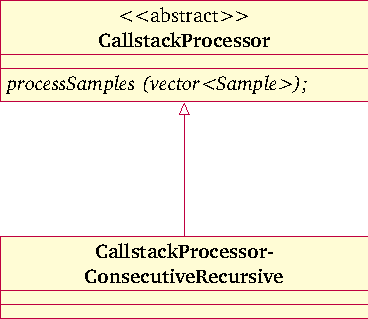
\includegraphics[width=0.35\textwidth]{figures/user-guide/tool-design-interpolate-callstack-processor.pdf}
  \caption{Call-stack processing related diagram classes.}
  \label{fig:tool_design_interpolate_callstackprocessor}
\end{figure}


With respect to the analysis of the call-stack, the \FOLDING tool has implemented this analysis through the \textsl{CallstackProcessor} related-classes that receives a set of \textsl{Sample} objects to explore.
Currently, the unique implementation available relies on aligning the call-stacks from the given samples and then exploring the call-stack frames at a given level whether consecutive samples refer to the same routine.
If the number of samples surpasses a given threshold, then applies it recursively to the next level until no more levels are available or the number of samples do not surpass the threshold.
